\clearpage
\section{GUI} \label{sec:GUI}

\begin{figure}[H]
\centering
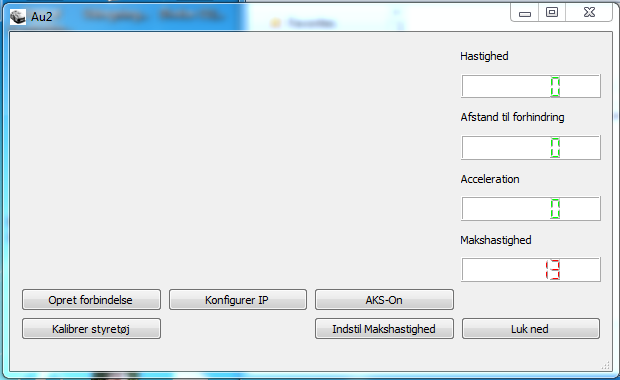
\includegraphics[width=\textwidth* 3/4,height=\textwidth* 9/20 ]{../fig/billeder/gui_start.png}
\caption{GUI hovedvindue}
\label{fig:GUI_hovedvindue}
\end{figure}

\subsection{Sekvensdiagrammer}

I denne sektion beskrives usecasene for GUI'en. Der er valgt at lave i alt 4 scenarier af UC1 hvor 3 af dem inkluderer fejl. Dette er gjort for at gøre det mere overskueligt, da et sekvensdiagram med en masse undtagelser hurtigt bliver forvirrende.På figur
\ref{fig:cd_uc1_succes_gui} ses sekvensdiagrammet over UC1 scenarie: succes.

\subsubsection{UC1 Succes}

\begin{figure}[H]
\centering
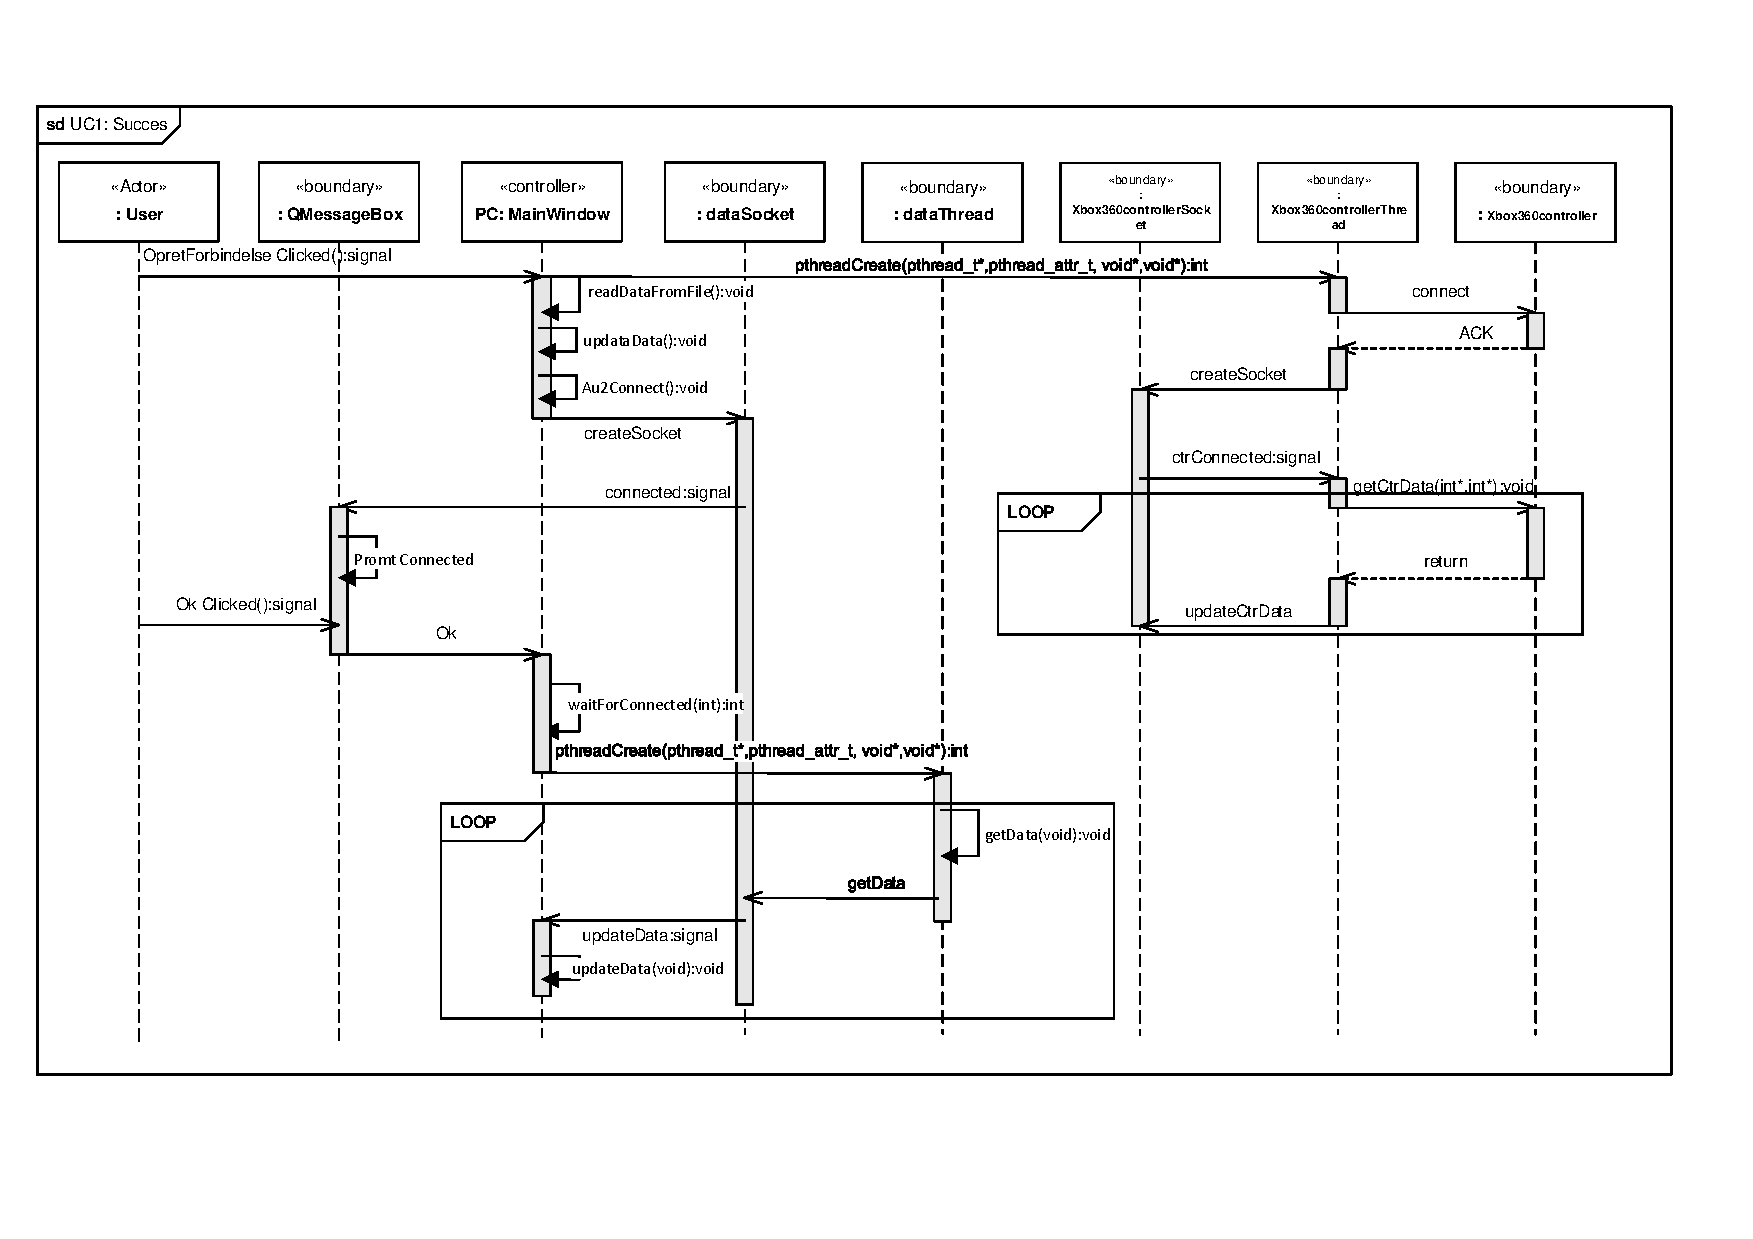
\includegraphics[width=\textwidth* 1,height=\textwidth* 1 ]{../fig/diagrammer/pc/sd_uc1_succes.pdf}
\caption{Sekvensdiagram over UC1 senarie:succes}
\label{fig:cd_uc1_succes_gui}
\end{figure}

Når usecasen startes klikker brugeren på ''Opret forbindelse'' på GUI'en. Herefter vil MainWindow starte Xbox360ControllerThread, som vil oprette en socketforbindelse mellem bilen og PC'en, til at streame controllerdata. Efterfølgende vil MainWindow læse indtastet data, som blev gemt i en fil sidste gang programmet lukkede ned og derefter opdatere vinduet. Nu vil MainWindow oprette en socket til at sende og modtage data fra og til bilen. Når socketforbindelsen er oprettet vil dataSocket sende et signal til MainWindow, som derved vil promte brugeren at forbindelsen er oprettet. Se figur \ref{fig:GUI_uc1_success}. Når brugeren lukker vinduet ved at klikke ''Ok'' venter MainWindow på at der er forbindelse for at derefter oprette dataThread som efterfølgende vil stå for at opdatere vinduet med hastig, afstand, acceleration osv. Det virker måske lidt dumt at vente på at der er forbindelse efter at der er givet signal om der er forbindelse. Dette skyldes at når brugeren trykker på ''Ok'' sættes en variabel til 1. Hvis forbindelsen senere mistes sættes denne variabel til 0, således dataThread ikke skriver til en socketforbindelse som ikke længere er aktiv. Kommer signalet om at forbindelsen ikke er oprettet inden for en given tid, vil programmet lave en fejl som det ses i figur....... Når dataThread har opdateret dataen, vil den give et signal til MainWindow om at der skal hentes nye data fra bilen. Det er derfor MainWindow som henter og sender data, men dataThread som opdatere selve dataen på GUI'en. Dette skyldes at QTcpsocket ikke kan køres i en seperat tråd som det gøres med Xbox360ControllerThread når der skal gives signaler. Der sker derfor en fejl i programmet når Xbox360 controlleren er forbundet og TCP forbindelsen mistes. Dette har der dog ikke været tid til at kigge nærmere på.  

\begin{figure}[H]
\centering
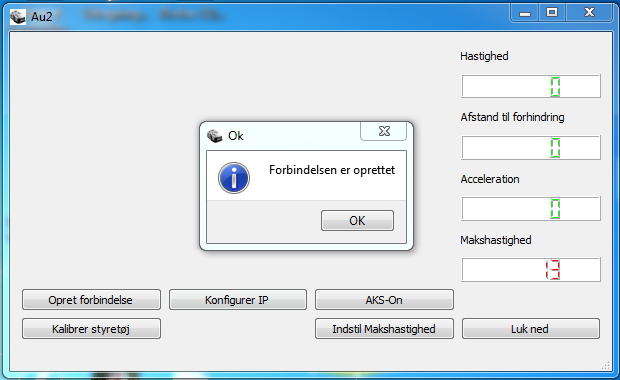
\includegraphics[width=\textwidth* 3/4,height=\textwidth* 9/20 ]{../fig/billeder/gui_uc1_success.png}
\caption{GUI UC1 succes}
\label{fig:GUI_uc1_success}
\end{figure}


\subsubsection{UC1 Error 1: Forbindelse kunne ikke oprettes}
I denne sektion beskrives fejlen, at der ikke kan oprettes forbindelse til bilen. Dette bliver som før beskrevet konkluderet i WaitForConnected(), som venter 1 sekund. Er der ikke givet signal inden deletes dataSocket og Xbox360ControllerSocket. Brugeren promtes med at forbindelsen ikke kunne oprettes. Se sekvensdiagrammet i figur \ref{fig:cd_uc1_error_1} og advarselsskiltet i figur \ref{fig:GUI_uc1_error_1}

\begin{figure}[H]
\centering
\includegraphics[width=\textwidth* 1,height=\textwidth* 1 ]{../fig/diagrammer/pc/sd_uc1_Error_1.pdf}
\caption{Sekvensdiagram over UC1 senarie:Error 1}
\label{fig:cd_uc1_error_1}
\end{figure}

\begin{figure}[H]
\centering
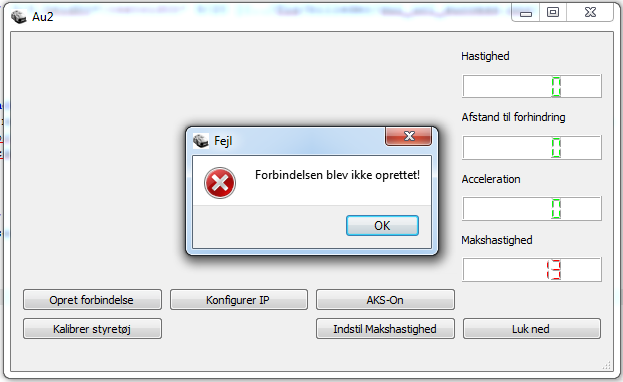
\includegraphics[width=\textwidth* 3/4,height=\textwidth* 9/20 ]{../fig/billeder/gui_uc1_error_1.png}
\caption{GUI UC1 Error 1}
\label{fig:GUI_uc1_error_1}
\end{figure}

\subsubsection{UC1 Error 2: Controller er ikke forbundet}
I denne sektion beskrives fejlen, at Xbox360-controlleren ikke er forbundet til PC'en. Når Xbox360controllerThread oprettes vil den spørge om controlleren er tilsluttet. Hvis den ikke er promtes bruger med at controlleren ikke er forbundet. Se sekvensdiagrammet i figur \ref{fig:cd_uc1_error_2} og advarselsskiltet i figur \ref{fig:GUI_uc1_error_2}

\begin{figure}[H]
\centering
\includegraphics[width=\textwidth* 1,height=\textwidth* 1 ]{../fig/diagrammer/pc/sd_uc1_Error_2.pdf}
\caption{Sekvensdiagram over UC1 senarie:Error 2}
\label{fig:cd_uc1_error_2}
\end{figure}

\begin{figure}[H]
\centering
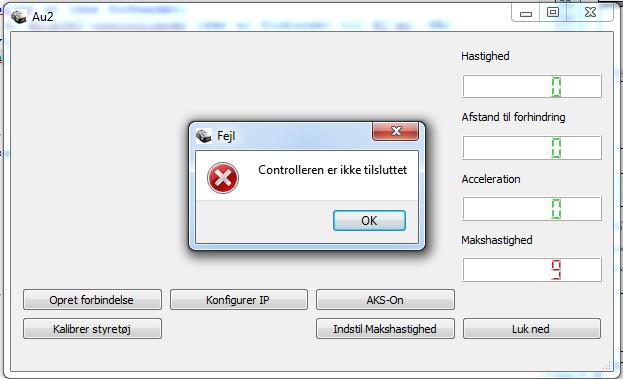
\includegraphics[width=\textwidth* 3/4,height=\textwidth* 9/20 ]{../fig/billeder/gui_uc1_error_2.png}
\caption{GUI UC1 Error 1}
\label{fig:GUI_uc1_error_2}
\end{figure}

\subsubsection{UC1 Error 3: Forbindelsen bliver afbrudt}
I denne sektion beskrives fejlen, at forbindelsen mellem bil og PC pludselig bliver afbrudt. dataSocket giver signal til MainWindow om at forbindelsen er afbrudt, som herefter giver besked til brugeren. Herefter stopper dataSocket med at opdatere data. Er controlleren forbundet og bliver denne forbindelse også afbrudt crasher programmet desværre. Denne fejl er beskrevet tidligere. Se sekvensdiagrammet i figur \ref{fig:cd_uc1_error_3} og advarselsskiltet i figur \ref{fig:GUI_uc1_error_3} 

\begin{figure}[H]
\centering
\includegraphics[width=\textwidth* 1,height=\textwidth* 1 ]{../fig/diagrammer/pc/sd_uc1_Error_3.pdf}
\caption{Sekvensdiagram over UC1 senarie:Error 3}
\label{fig:cd_uc1_error_3}
\end{figure}

\begin{figure}[H]
\centering
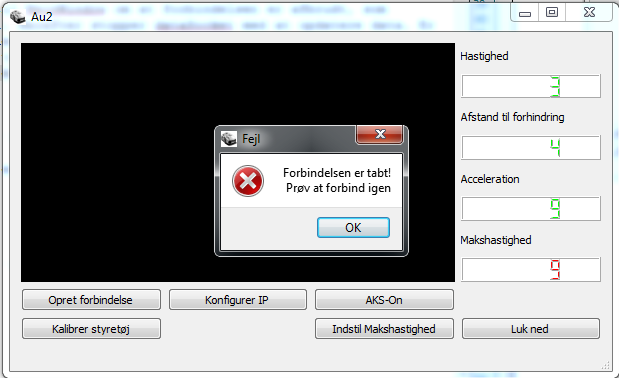
\includegraphics[width=\textwidth* 3/4,height=\textwidth* 9/20 ]{../fig/billeder/gui_uc1_error_3.png}
\caption{GUI UC1 Error 3}
\label{fig:GUI_uc1_error_3}
\end{figure}

\subsubsection{UC8: Konfigurer IP-adresse}
For at aktivere usecase 8 trykker bruger på ''Konfigurer IP''. Herefter åbner MainWindow en inputdialog som bruger indtaster IP-adressen i og efterfølgende trykker ''Ok''. Se sekvensdiagrammet i figur \ref{fig:cd_uc8} og indputdialogen i figur \ref{fig:GUI_uc8} 

\begin{figure}[H]
\centering
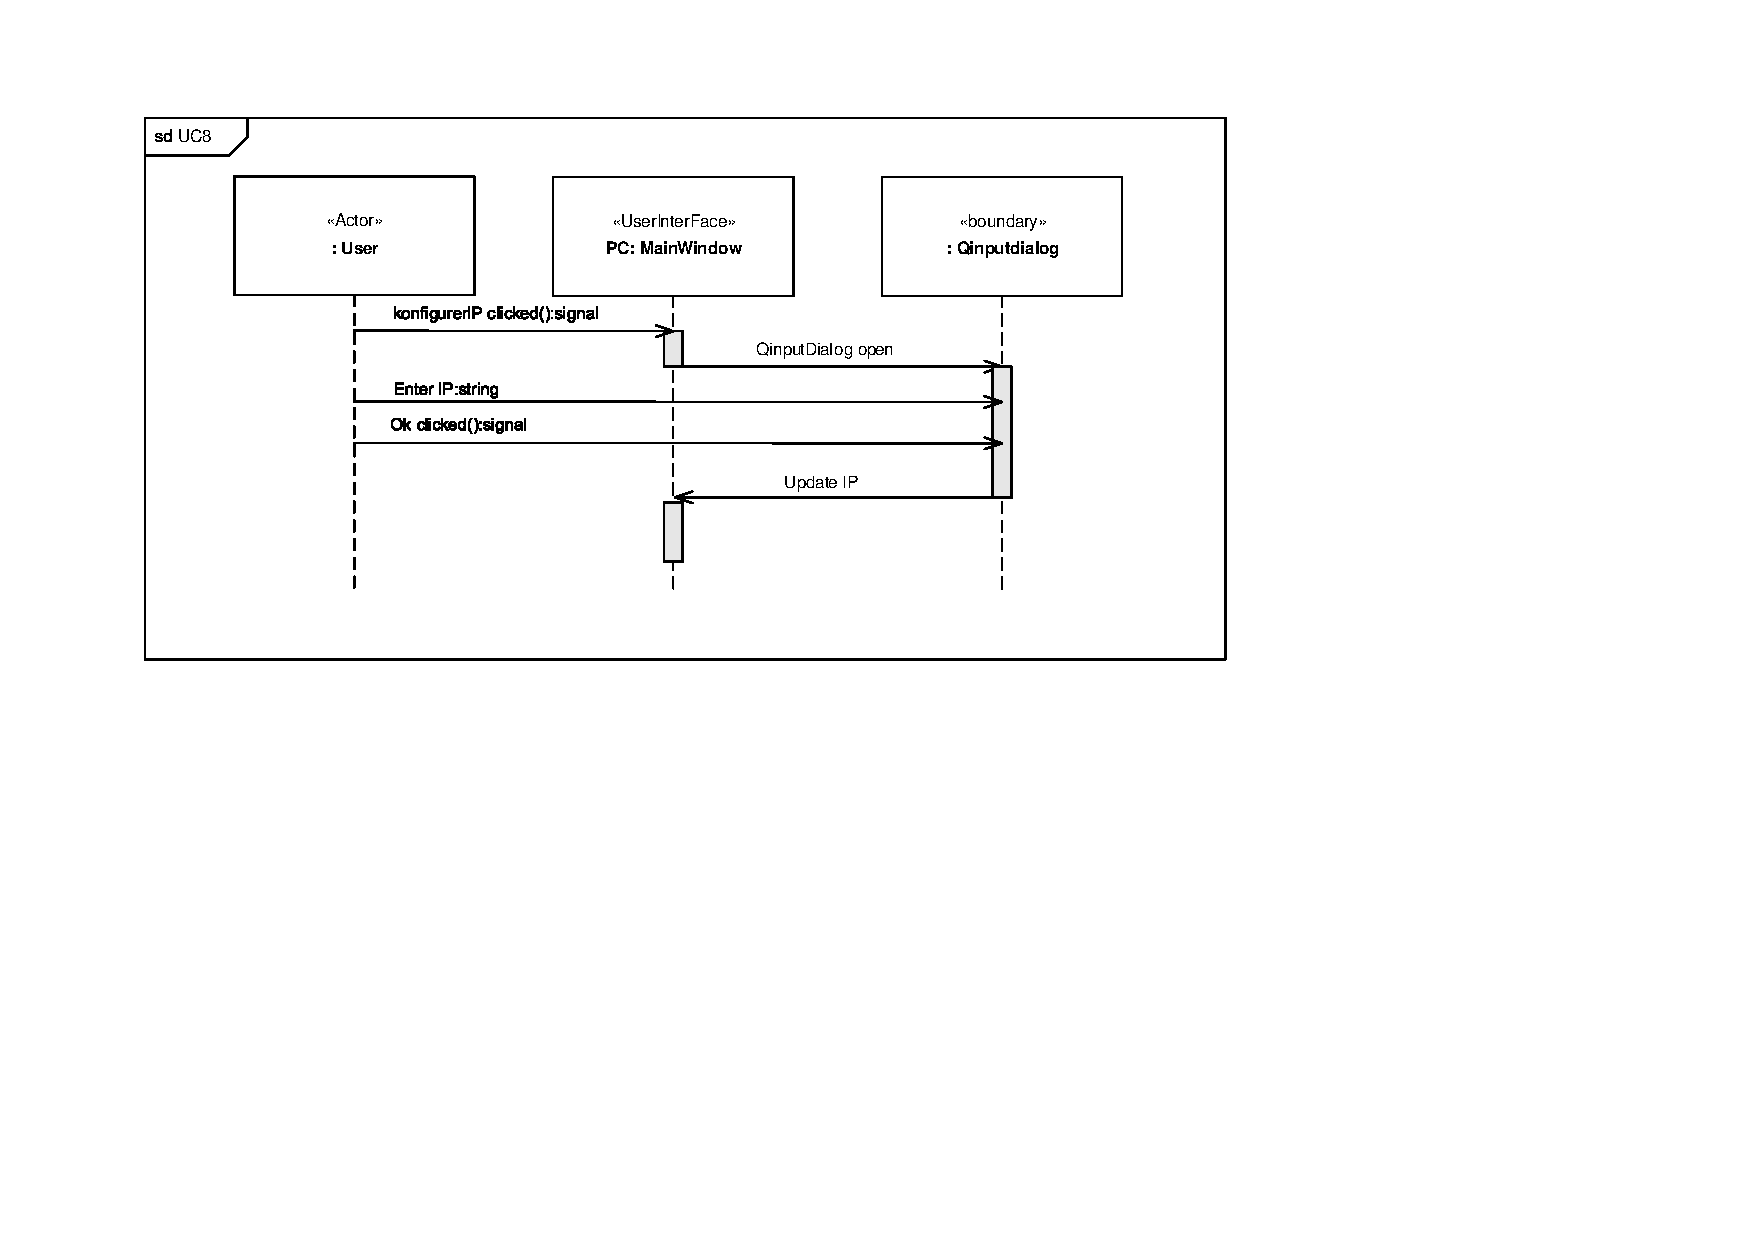
\includegraphics[width=\textwidth* 2/3,height=\textwidth* 4/10 ]{../fig/diagrammer/pc/sd_uc8.pdf}
\caption{Sekvensdiagram over UC8}
\label{fig:cd_uc8}
\end{figure}

\begin{figure}[H]
\centering
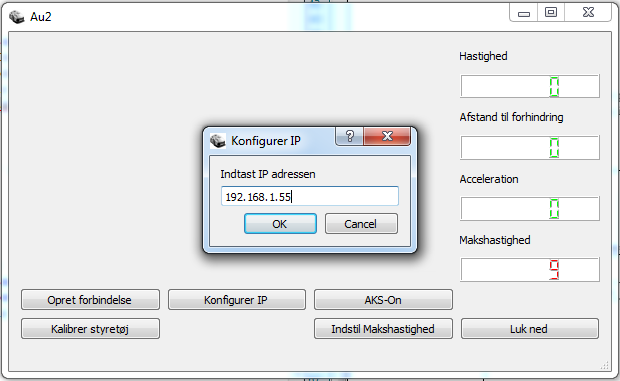
\includegraphics[width=\textwidth* 3/4,height=\textwidth* 9/20 ]{../fig/billeder/gui_uc8.png}
\caption{GUI UC8}
\label{fig:GUI_uc8}
\end{figure}

\subsubsection{UC9: Tænd/sluk AKS}
For at aktivere usecase 9 trykker bruger på ''AKS-On''.
Når bruger trykker på denne ændres teksten til ''AKS-Off''. Er teksten i forvejen ''AKS-Off'' ændres denne til ''AKS-On''. En variabel i MainWindow opdateres og gived med til bilen næste gang data bliver opdateret i UC1. Se sekvensdiagrammet i figur \ref{fig:cd_uc9} og indputdialogen i figur \ref{fig:GUI_uc9}

\begin{figure}[H]
\centering
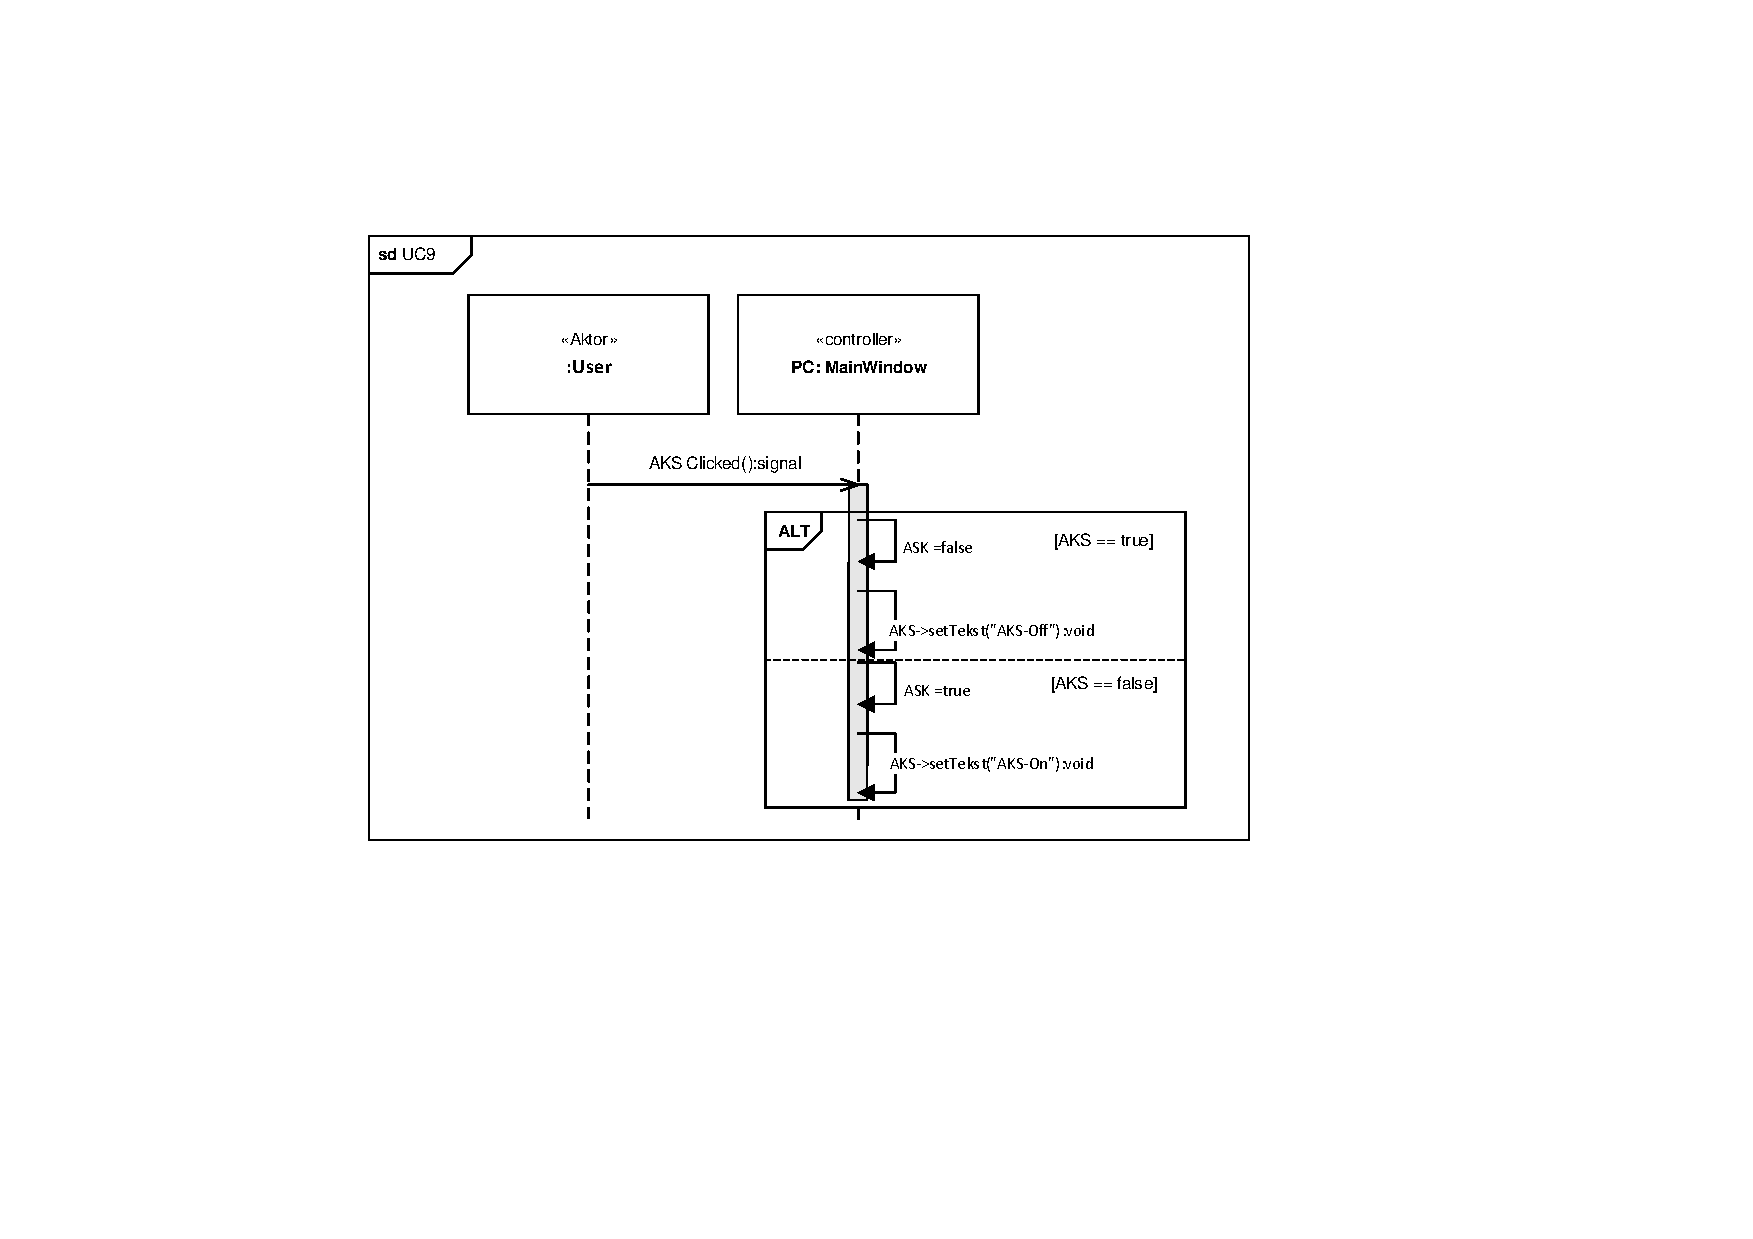
\includegraphics[width=\textwidth* 2/3,height=\textwidth* 4/10 ]{../fig/diagrammer/pc/sd_uc9.pdf}
\caption{Sekvensdiagram over UC9}
\label{fig:cd_uc9}
\end{figure}

\begin{figure}[H]
\centering
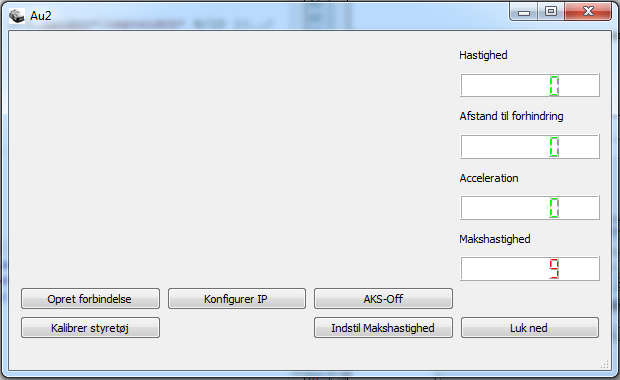
\includegraphics[width=\textwidth* 3/4,height=\textwidth* 9/20 ]{../fig/billeder/gui_uc9.png}
\caption{GUI UC9}
\label{fig:GUI_uc9}
\end{figure}

\subsubsection{UC10: Indstil makshastighed}
For at aktivere usecase 10 trykker bruger på ''Indstil makshastighed''.
MainWindow åbner en inputdialog hvor i bruger indtaster et tal mellem 0 og 10. Inputdialogen accepterer ikke indtastninger uden for dette interval. Se sekvensdiagrammet i figur \ref{fig:cd_uc10} og indputdialogen i figur \ref{fig:GUI_uc10}

\begin{figure}[H]
\centering
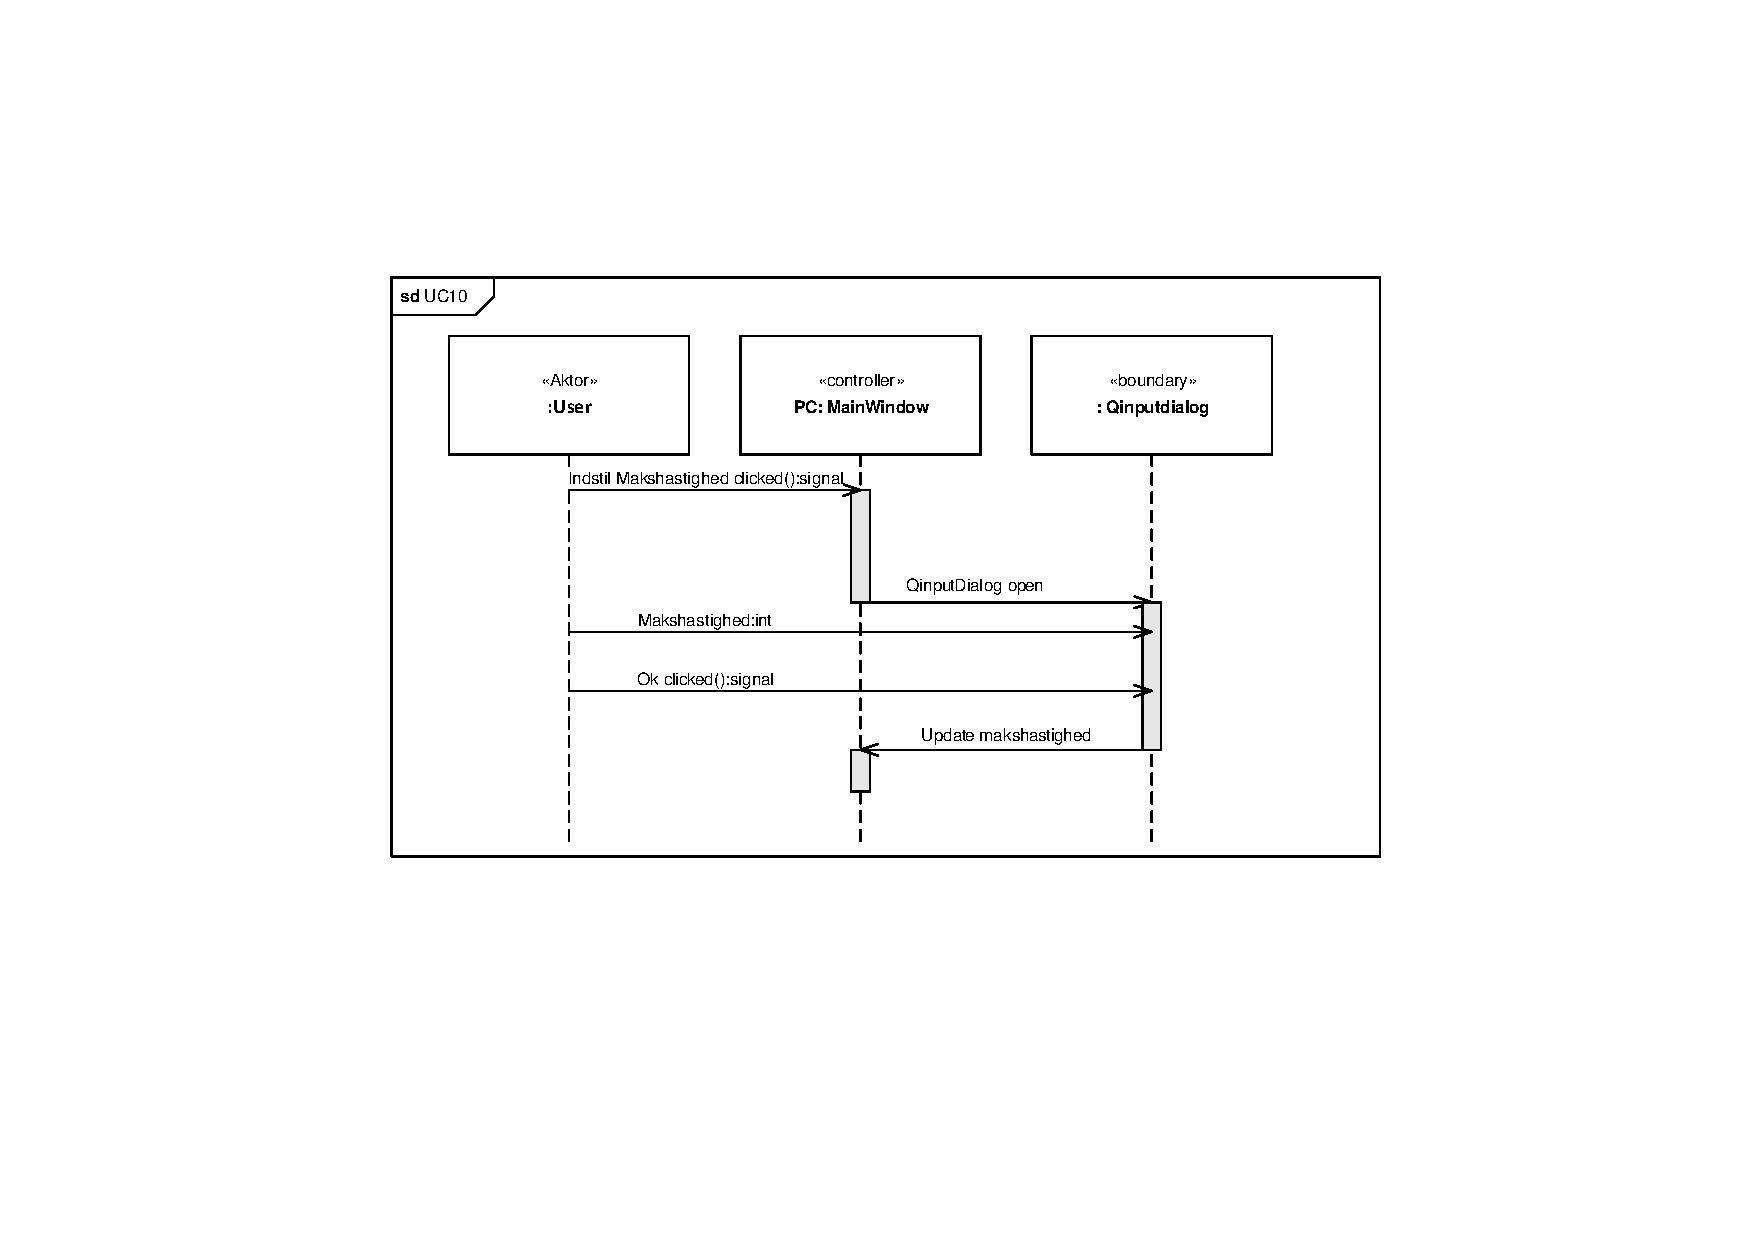
\includegraphics[width=\textwidth* 2/3,height=\textwidth* 4/10 ]{../fig/diagrammer/pc/sd_uc10.pdf}
\caption{Sekvensdiagram over UC10}
\label{fig:cd_uc10}
\end{figure}

\begin{figure}[H]
\centering
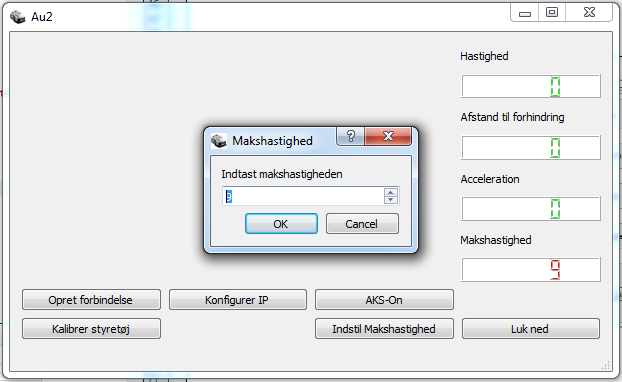
\includegraphics[width=\textwidth* 3/4,height=\textwidth* 9/20 ]{../fig/billeder/gui_uc10.png}
\caption{GUI UC10}
\label{fig:GUI_uc10}
\end{figure}

\subsubsection{UC11: Kalibrer styretøj}
For at aktivere usecase 11 trykker bruger på ''Kalibrer styretøj''.
MainWindow åbner en inputdialog hvor i bruger indtaster et tal mellem -50 og 50. Inputdialogen accepterer ikke indtastninger uden for dette interval. Se sekvensdiagrammet i figur \ref{fig:cd_uc11} og indputdialogen i figur \ref{fig:GUI_uc11}

\begin{figure}[H]
\centering
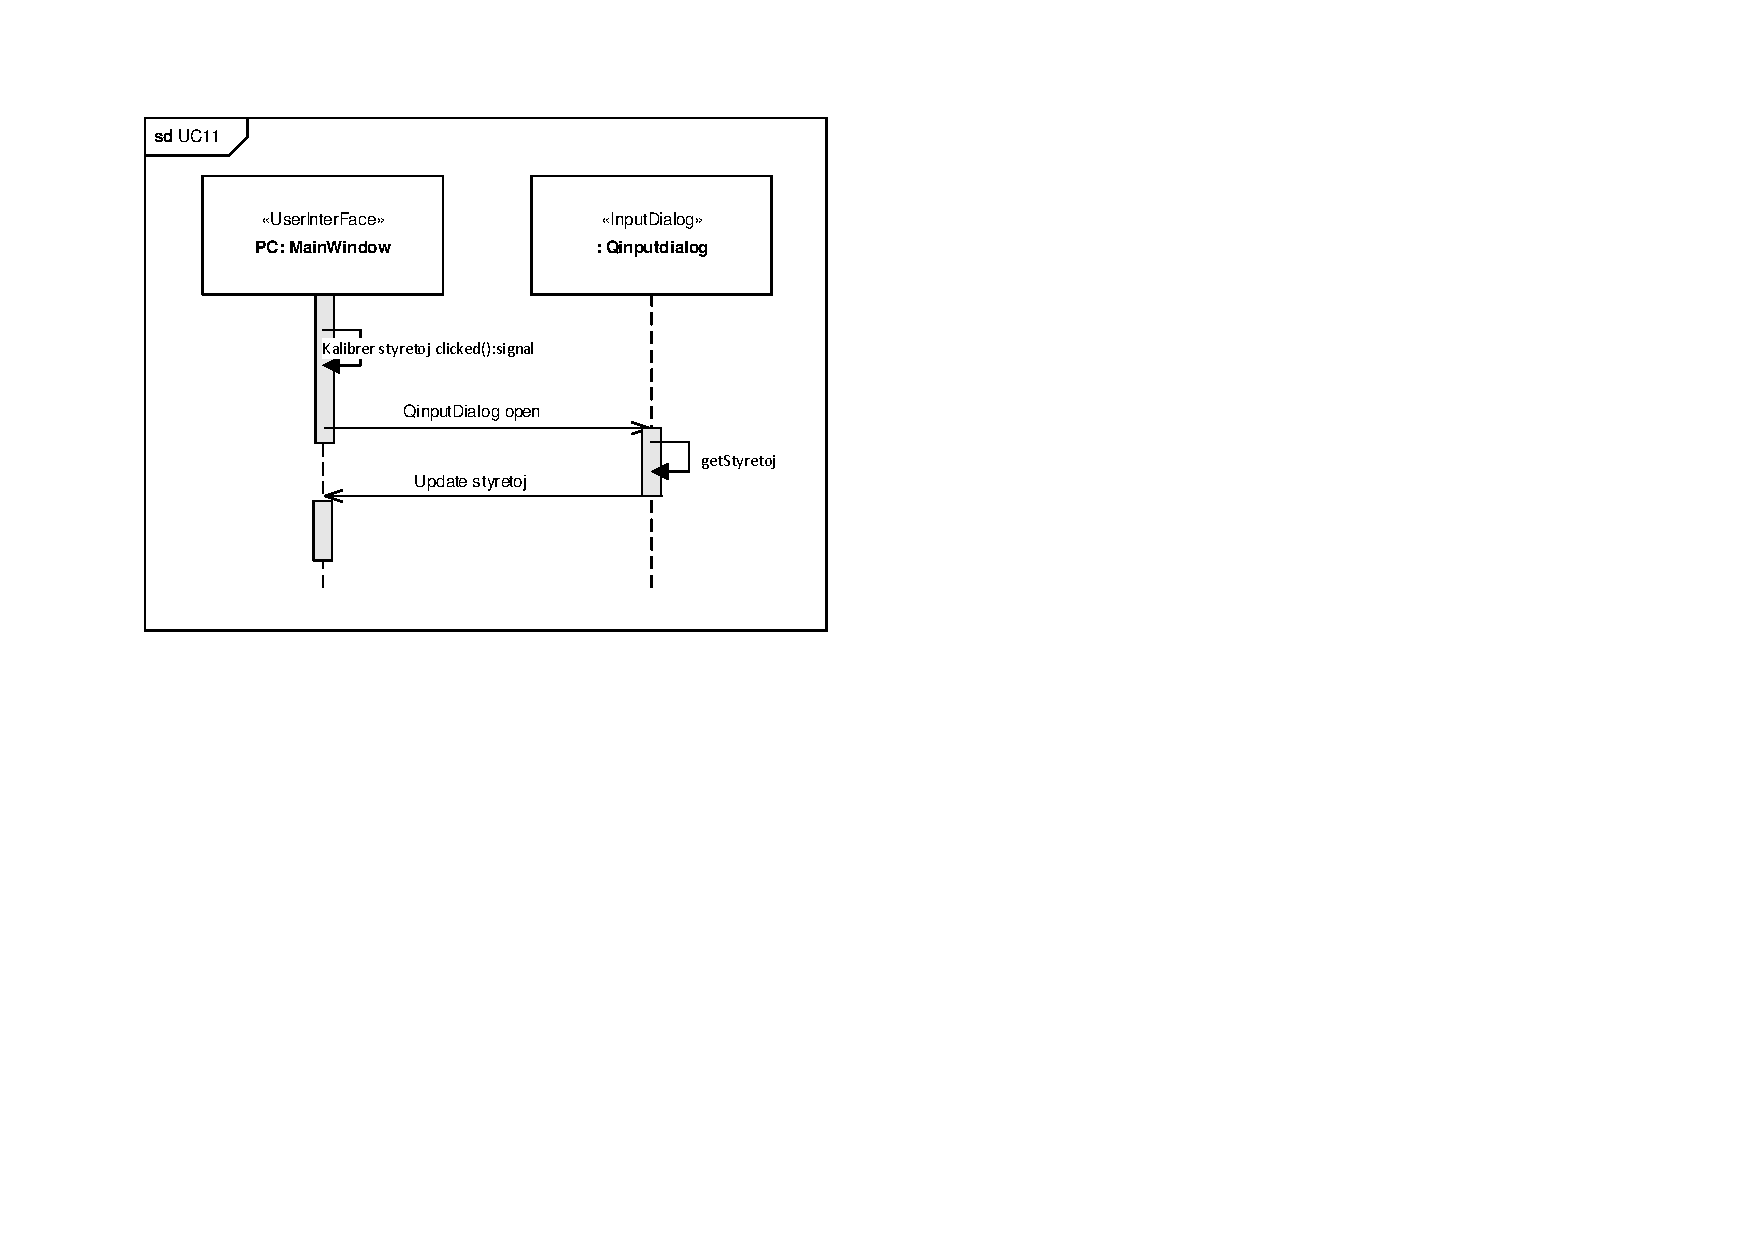
\includegraphics[width=\textwidth* 2/3,height=\textwidth* 4/10 ]{../fig/diagrammer/pc/sd_uc11.pdf}
\caption{Sekvensdiagram over UC11}
\label{fig:cd_uc11}
\end{figure}

\begin{figure}[H]
\centering
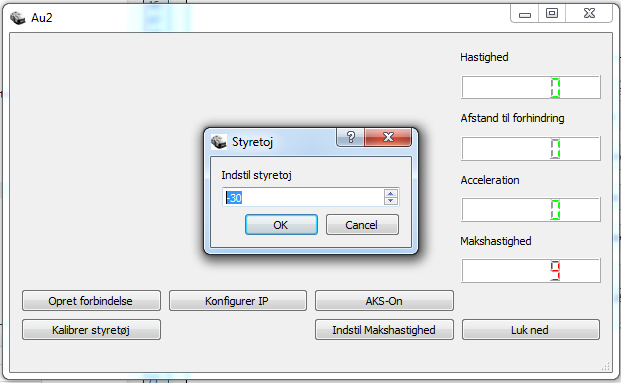
\includegraphics[width=\textwidth* 3/4,height=\textwidth* 9/20 ]{../fig/billeder/gui_uc11.png}
\caption{GUI UC11}
\label{fig:GUI_uc11}
\end{figure}

\subsubsection{UC12: Afbryd system}
For at aktivere usecase 11 trykker bruger på ''Luk ned''.
dataSocket beder bilen om at lukke ned og bilen svarer med et ACK. Modtages der ikke et ACK giver MainWindow bruger besked om at bilen ikke kan lukke ned. Se sekvensdiagrammet i figur \ref{fig:cd_uc11} og advarslen i figur \ref{fig:GUI_uc11}

\begin{figure}[H]
\centering
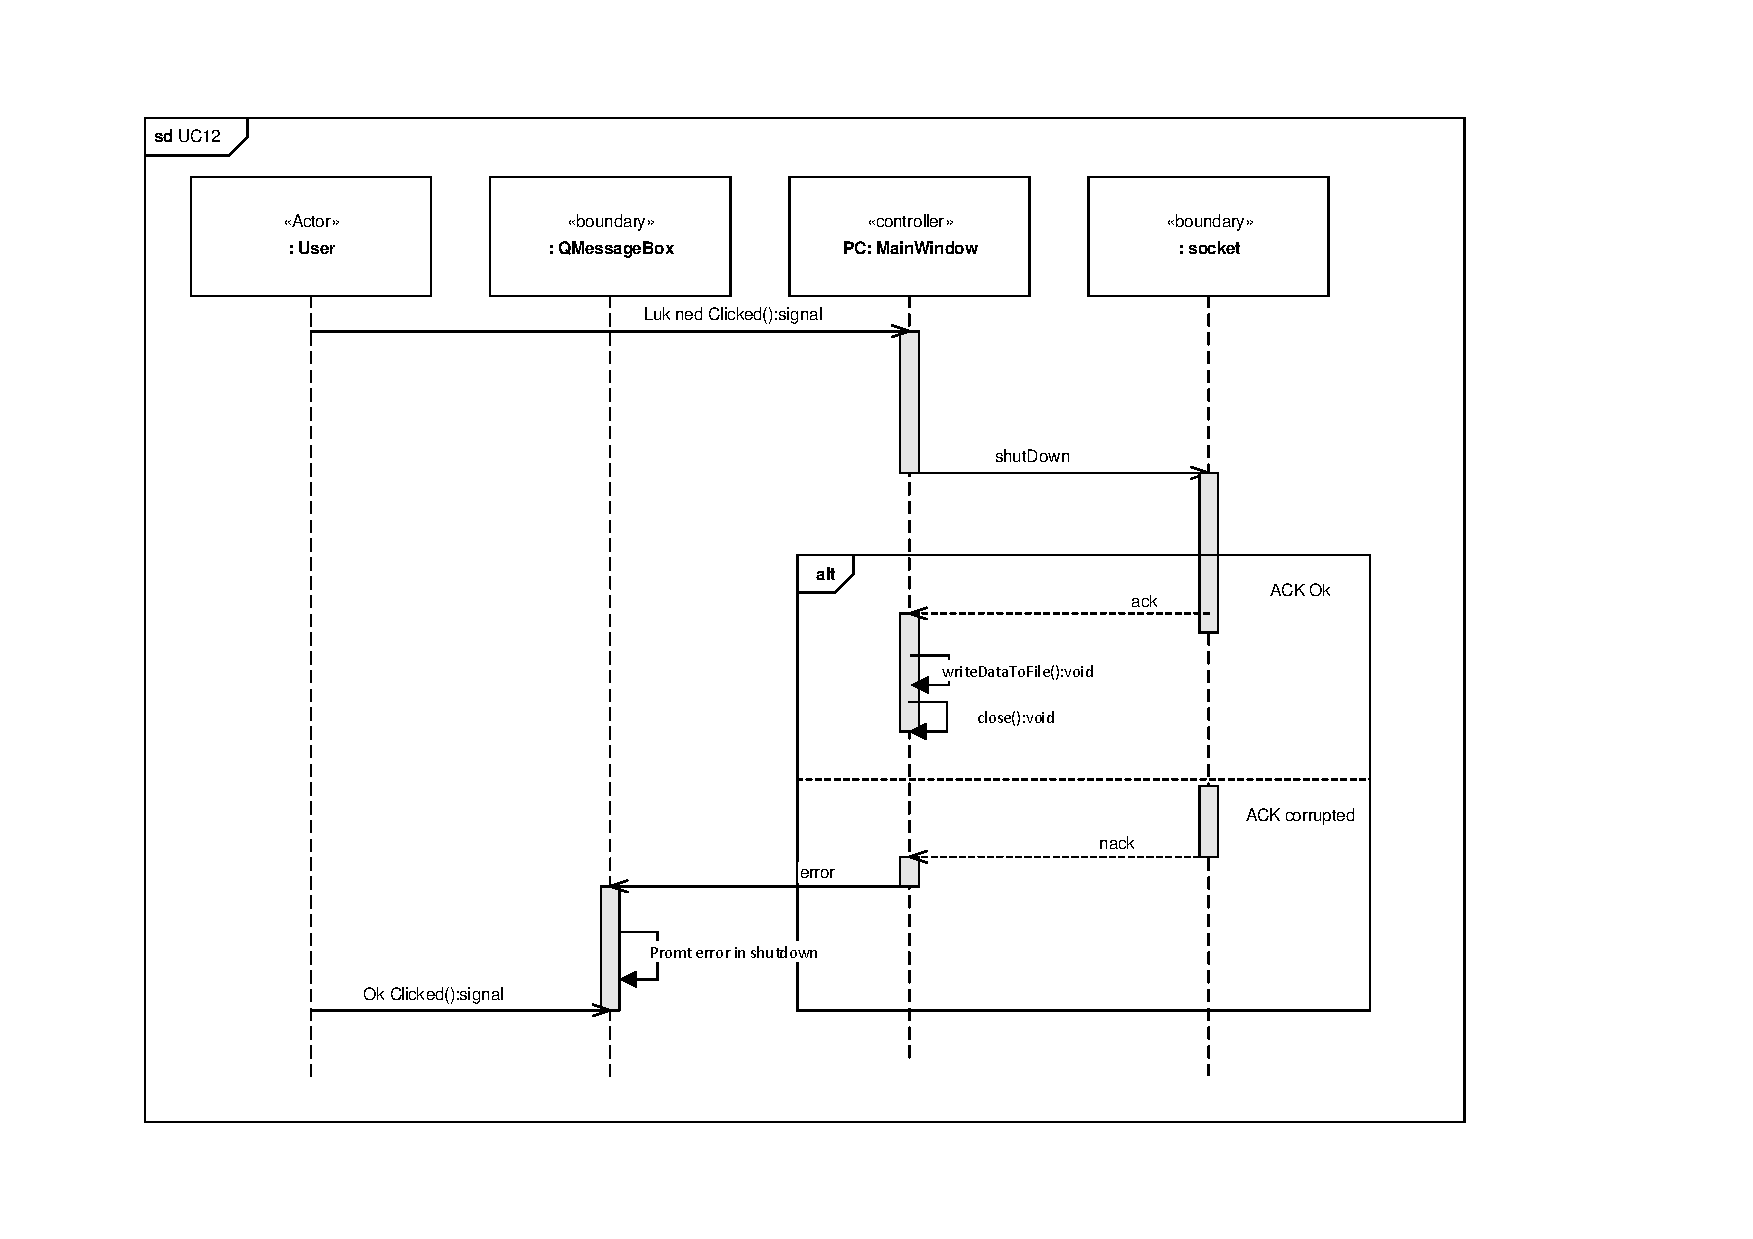
\includegraphics[width=\textwidth* 2/3,height=\textwidth* 4/10 ]{../fig/diagrammer/pc/sd_uc12.pdf}
\caption{Sekvensdiagram over UC12}
\label{fig:cd_uc12}
\end{figure}

\begin{figure}[H]
\centering
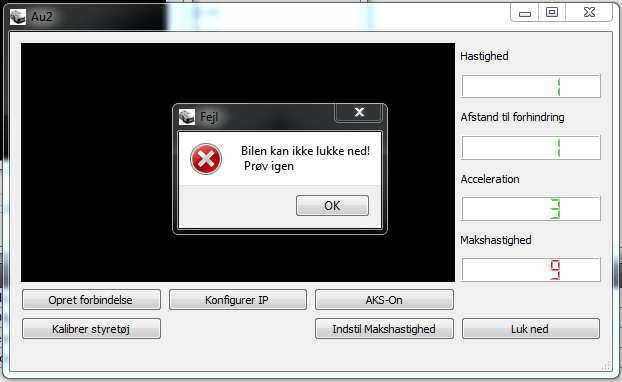
\includegraphics[width=\textwidth* 3/4,height=\textwidth* 9/20 ]{../fig/billeder/gui_uc12.png}
\caption{GUI UC12}
\label{fig:GUI_uc12}
\end{figure}


\subsection{Klassebeskrivelse}
I denne sektion vil der blive beskrevet klassen MainWindow og XboxController. MainWindow er GUI'ens hoved klasse hvor i alt styres fra. XboxController er controllerens klasse som MainWindow bruger til at streame controllerdata fra.

\begin{figure}[H]
\centering
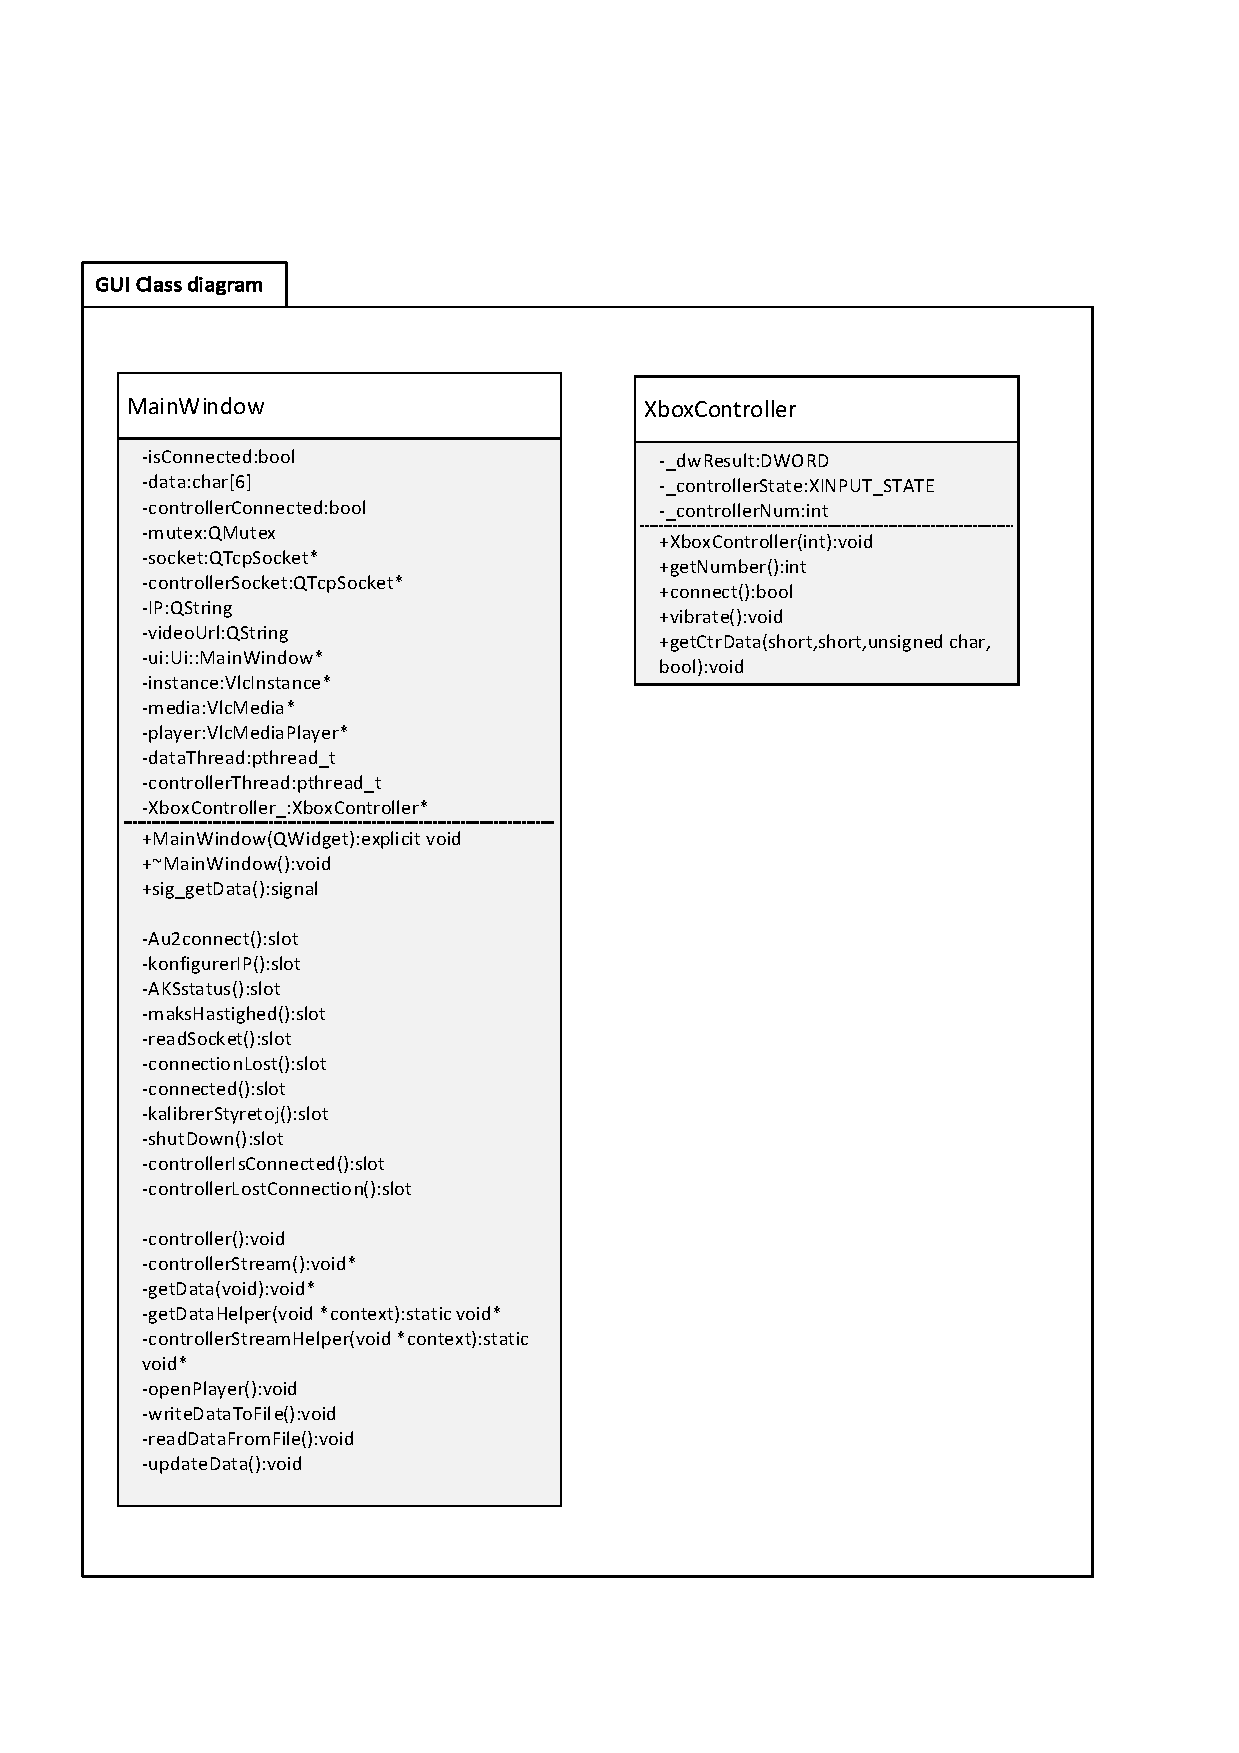
\includegraphics[width=\textwidth* 9/10]{../fig/diagrammer/pc/gui_classdiagram.pdf}
\caption{Klasse diagram over GUI}
\label{fig:cd_gui}
\end{figure}

\textbf{Attributter for MainWindow}

\begin{table}[H]
\begin{tabularx}{\textwidth}{| Z | Z | L{10cm} |} \hline
Navn & Type & Beskrivelse \\\hline
\texttt{isConnected}         & \texttt{bool}           &Bliver brugt til at angive om socket har forbindelse til bilen eller ej \\\hline
\texttt{data}                & \texttt{char[6]}        &Char array som indeholder: Hastighed, Makshastighed, AKS-status, Styretøj, Acceleration og Afstand\\\hline
\texttt{controller -Connected} & \texttt{bool}           &Bruges til at angive om Xbox360-controlleren er forbundet eller ej\\\hline
\texttt{mutex}               & \texttt{QMutex*}        &Bruges til at låse således data kun kan tilgås af en tråd af gangen\\\hline
\texttt{socket}              & \texttt{QTcpSocket*}    &Er selve datasocket instancen\\\hline
\texttt{controller -Socket}    & \texttt{QTcpSocket*}    &Er selve controllerSocket instansen\\\hline
\texttt{IP}                  & \texttt{QString}        &Indeholder IP-adressen på bilen\\\hline
\texttt{videoURL}            & \texttt{QString}        &Indeholder adressen på videostreamet fra bilen\\\hline
\texttt{ui::Ui}              & \texttt{MainWindow*}    &Selve GUI'en\\\hline
\texttt{instance}            & \texttt{VlcInstance*}   &Bruges til at afspille videostream\\\hline
\texttt{media}               & \texttt{VlcMedia*}      &Bruges til at afspille videostream\\\hline
\texttt{player}              & \texttt{VlcMediaPlay -er*}&Bruges til at afspille videostream\\\hline
\texttt{dataThread}          & \texttt{p\_thread\_t}     &Er selve data tråden\\\hline
\texttt{controller -Thread}    & \texttt{p\_thread\_t}     &Er selve controller tråden\\\hline
\texttt{XboxControl -ler\_}     & \texttt{XboxControl -ler*}&En instance af Xbox360-controlleren\\\hline

\end{tabularx}
\caption{Attributter for klassen MainWindow}
\label{table:attr_distancesensor}
\end{table}



